\documentclass[11pt,a4paper]{article}
\usepackage[utf8]{inputenc}
\usepackage[T1]{fontenc}
\usepackage{amsmath}
\usepackage{amsfonts}
\usepackage{amssymb}
\usepackage{makeidx}
\usepackage{graphicx}
\usepackage{gensymb}
\usepackage{breqn}
%\usepackage{mathptmx}
\usepackage{newpxtext}
\usepackage[T1]{fontenc}
\author{Karthik J}
\date{}
\title{\vspace{-50pt}\textsc{Calibration of Si diode\\as a Temperature Sensor}}
\begin{document}
	\maketitle
	\section{Platinum wire Thermometers}
	A \textbf{thermometer} works based on the variation of some property of any material with temperature. The \textbf{platinum resistance thermometer} works on the principle of variation of the electrical resistance of high purity platinum wire with temperature. 
	\subsection{Advantages of Platinum wire thermometer}
	\begin{enumerate}
		\item 	good temperature coefficient of
		resistance ($\alpha$),
		\item 	the variation of its resistance with temperature is almost linear over a wide range of temperature.
	\end{enumerate}
	A platinum resistor with a resistance of 100 $\Omega$ at $0\degree$C is called \textbf{Pt100}. The resistance of this Pt100 thermometer increases by 0.39 $\Omega$ for every 1$\degree$C rise in temperature.
	
	\section{Diode thermometer}
	
	A pn junction diode can also be used as a thermometer. A small current (about 1 to 2 mA) is passed through a diode in the forward direction, and the voltage drop is measured across the diode. 
	
	The current and voltage across a p-n junction diode is given by the Shockley equation:
	\begin{equation}\label{shockley}
		I = I_0 \left[\exp \left( \dfrac{qV}{k_B T} \right) - 1\right]
	\end{equation}
	where \\
	\begin{tabular}{ccl}
		$I_0$ & $\rightarrow$& \text{reverse saturation current}\\
		$k_B$ & $\rightarrow$ & \text{Boltzmann's constant}\\
		$q$&  $\rightarrow$& \text{elementary charge}\\
		$V$ & $\rightarrow$& \text{forward voltage across the diode}\\
		$I$ &$\rightarrow$& \text{forward current through the diode}\\
		$T$ &$\rightarrow$& \text{temperature}\\
	\end{tabular}
	\vspace{10pt}\\
	The reverse saturation current, $I_0$, is not constant for a given device, but varies with temperature; usually more significantly than $\left(\dfrac{k_B T}{q}\right)$, so that \emph{$V$ decreases as $T$ increases}.
	\begin{equation}\label{reverse_current}
		I_{0}=A \exp \left(-\frac{E_{g}}{2 k_{B} T}\right)
	\end{equation}
	where $A$ depends primarily on the geometry and doping of the junction region and $E_g$ is the semiconductor band gap. Solving equations \ref{shockley} \& \ref{reverse_current} for the voltage $V$,
	\begin{equation}
		V_{D}=\frac{\ln \left(\frac{I}{A}\right) 2 k_{B} T+E_{g}}{q}
	\end{equation}
	If the current through the diode is held constant, there is now a simple linear relationship between voltage and temperature. If the diodes we will use were ideal, this expression would be all we need. For real diodes, the functional form is still quite
	linear, e.g.,
	\begin{equation}\label{VT}
	V = a - bT
	\end{equation}
	If the current through the diode is kept constant, this \emph{forward voltage decreases} as the temperature increases, nearly linearly over a limited temperature region. This decrease is measurable with a digital voltmeter. The diode thermometer can be used for controlling the temperature. The forward voltage of a diode changes with the age of the diode. For precise measurements of temperature, a diode is almost never used. 
	
	The temperature variation of the forward voltage of a silicon diode at a constant current is studied in this experiment. The temperature is measured with a Pt100 resistance thermometer.
	
	\begin{figure}[!htb]
		\centering
		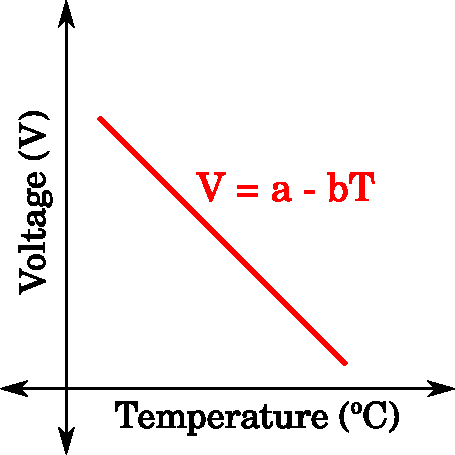
\includegraphics[scale=0.6]{VT}
		\caption{Variation of forward Voltage drop with Temperature}
	\end{figure}
	
	The graph of forward voltage drop against temperature (figure 1) can be fitted to a linear equation \ref{VT} where $a$ and $b$ are constants which can be determined from the fit curve.
	This can be used to determine the temperature, when a constant current is flowing across the diode.
\end{document}